\documentclass{beamer}
\usepackage[UTF8,noindent]{ctexcap}  
%\documentclass[handout,t]{beamer}

\batchmode
% \usepackage{pgfpages}
% \pgfpagesuselayout{4 on 1}[letterpaper,landscape,border shrink=5mm]

\usepackage{amsmath,amssymb,enumerate,epsfig,bbm,calc,color,ifthen,capt-of,multimedia,hyperref}

\usetheme{Berlin}
\usecolortheme{sustech}
\usepackage{caption}
\usepackage{subcaption}
\usepackage{graphicx}
\usepackage{color}
\usepackage{amssymb}

\title{Natural Water Simulation}
\author{Team Wavy}
\institute{School of Data and Computer Science(SYSU)}
\date{\today}

%\pgfdeclareimage[height=0.5cm]{sustech-logo}{logo.png}
\logo{\pgfuseimage{sustech-logo}\hspace*{0.3cm}}

\AtBeginSection[]
{
  \begin{frame}<beamer>
    \frametitle{Outline}
    \tableofcontents[currentsection]
  \end{frame}
}
\beamerdefaultoverlayspecification{<+->}
% -----------------------------------------------------------------------------
\begin{document}
% -----------------------------------------------------------------------------

\frame{\titlepage}

\section[Outline]{}
\begin{frame}{Outline}
  \tableofcontents
\end{frame}

% -----------------------------------------------------------------------------
\section{Introduction}
\subsection{Current Work}
%%%%%%%%%%%%%%%%%%%%%%%%%%%%%%%%%%%%%%%%%%%%%
\begin{frame}{Some main references}
  %\begin{columns}[T] % align columns
    %\begin{column}<0->{.40\textwidth}
    %  \begin{figure}[thpb]
    %    \centering
    %    \resizebox{1\linewidth}{!}{
    %    \includegraphics{figures/sustech.pdf}
    %    }
    %    \includegraphics[scale=1.0]{figurefile}
    %    \caption{SUSTech Campus}
    %    \label{fig:campus}
    %  \end{figure}
    %\end{column}%
    %\hfill%
    %\begin{column}<0->{.65\textwidth}
      \begin{itemize}
        \item<1-> \href{http://w3.oc.ntu.edu.tw/chap7/chap7s2.htm}{A lecture note of ocean waves simulation of NTU} 
        \item<2-> \href{http://cdmd.cnki.com.cn/Article/CDMD-10590-1017812561.htm}{Haibo Ma. Research and application of real-time wave simulation algorithm [D]. Shenzhen University, 2017.}
        \item<3-> \href{http://pub.ist.ac.at/group_wojtan/projects/2017_Jeschke_WaterWavePackets/wavepackets_author.pdf}{Jeschke S, Wojtan C. Water wave packets[J]. Acm Transactions on Graphics, 2017, 36(4):1-12.}
        \item<4-> \href{http://kns.cnki.net/KCMS/detail/detail.aspx?dbcode=CMFDanddbname=CMFD201701andfilename=1016765176.nhanduid=WEEvREcwSlJHSldRa1FhcTdWajFtZkFNbGZQYWkvYUlrbXkvUjdZRGJhST0=$9A4hF_YAuvQ5obgVAqNKPCYcEjKensW4ggI8Fm4gTkoUKaID8j8gFw!!andv=MzE2NjJDVVJMS2ZZZWRuRkNqaFZyektWRjI2R0xTK0c5RExxWkViUElSOGVYMUx1eFlTN0RoMVQzcVRyV00xRnI=}{Fuding Fan. Real time rendering algorithm for virtual ocean multi scene elements [D]. Yanshan University, 2016.}
        \item<5-> \href{http://visualcomputing.ist.ac.at/publications/2018/WSW/}{Stefan J, Tomas S, Matthias M.F, Nuttapong C, Miles M, Chris W. Water Surface Wavelets[J]. ACM Transactions on Graphics, 2017, 37(4):1-13.}  
      \end{itemize}
    %\end{column}
  %\end{columns}
\end{frame}
%%%%%%%%%%%%%%%%%%%%%%%%%%%%%%%%%%%%%%%%
%\subsection{}
\begin{frame}{Applications}
  It's just everywhere!
  \begin{itemize}
    \item Ads
    \item Cartoon
  \end{itemize}

  \begin{figure}[thpb]
    \centering
    \resizebox{1\linewidth}{!}{
        %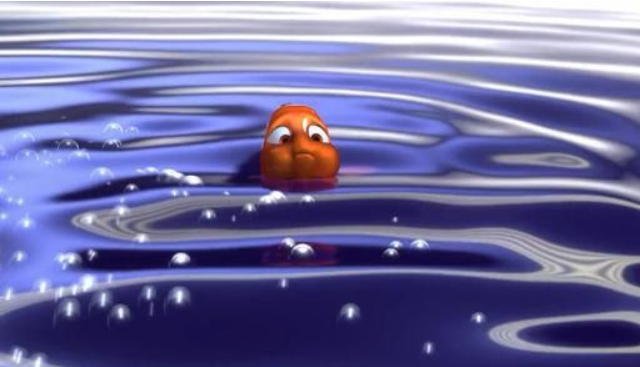
\includegraphics{figures/pic1.png}
        \begin{subfigure}[t]{0.5\textwidth}
        \centering
        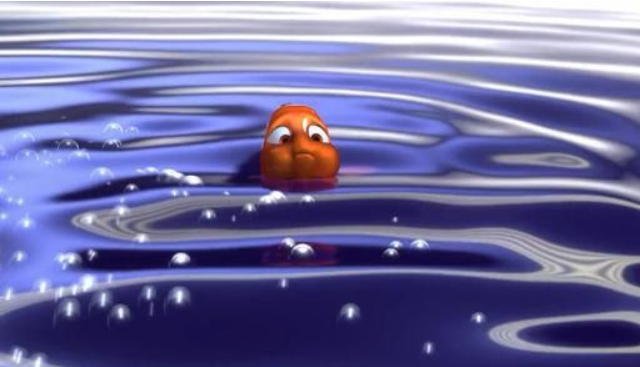
\includegraphics[width=1\textwidth]{figures/pic1.png}
        \subcaption*{The first film}
        \end{subfigure}
        \quad
        \begin{subfigure}[t]{0.5\textwidth}
        \centering
        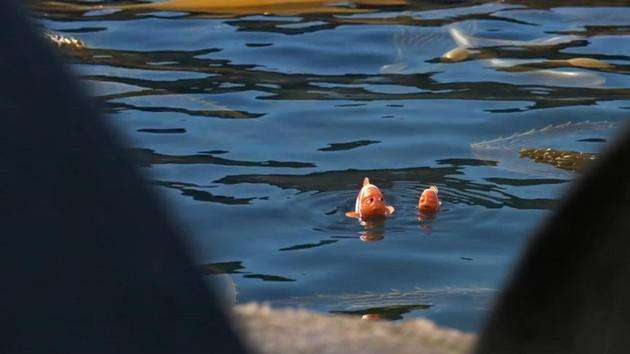
\includegraphics[width=1\textwidth]{figures/pic2.jpg}
        \subcaption*{The second film}
        \end{subfigure}
    }
    \caption*{\emph{Finding Nemo}({\fangsong 海底总动员})}
  \label{fig:1}
  \end{figure}
\end{frame}

\begin{frame}{Applications}
  \begin{itemize}
    \item Computer games(Lifelike effect makes us absorbed!)
  \end{itemize}
  
  \begin{figure}[thpb]
    \centering
    \resizebox{1\linewidth}{!}{
        %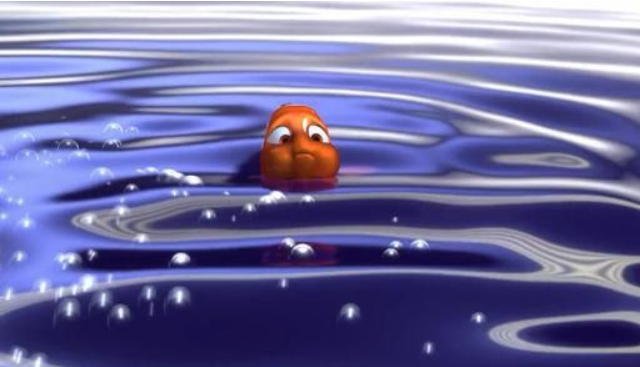
\includegraphics{figures/pic1.png}
        \begin{subfigure}[t]{0.5\textwidth}
        \centering
        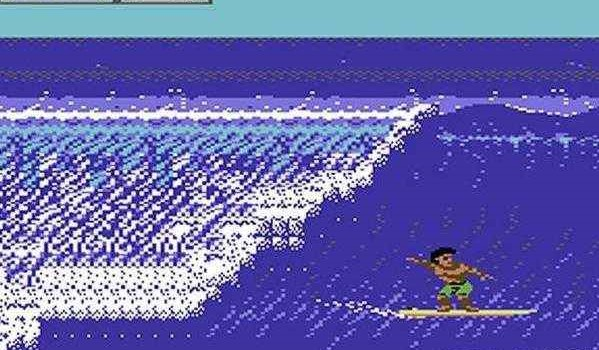
\includegraphics[width=1\textwidth]{figures/pic3.jpg}
        \subcaption*{2D games?}
        \end{subfigure}
        \quad
        \begin{subfigure}[t]{0.5\textwidth}
        \centering
        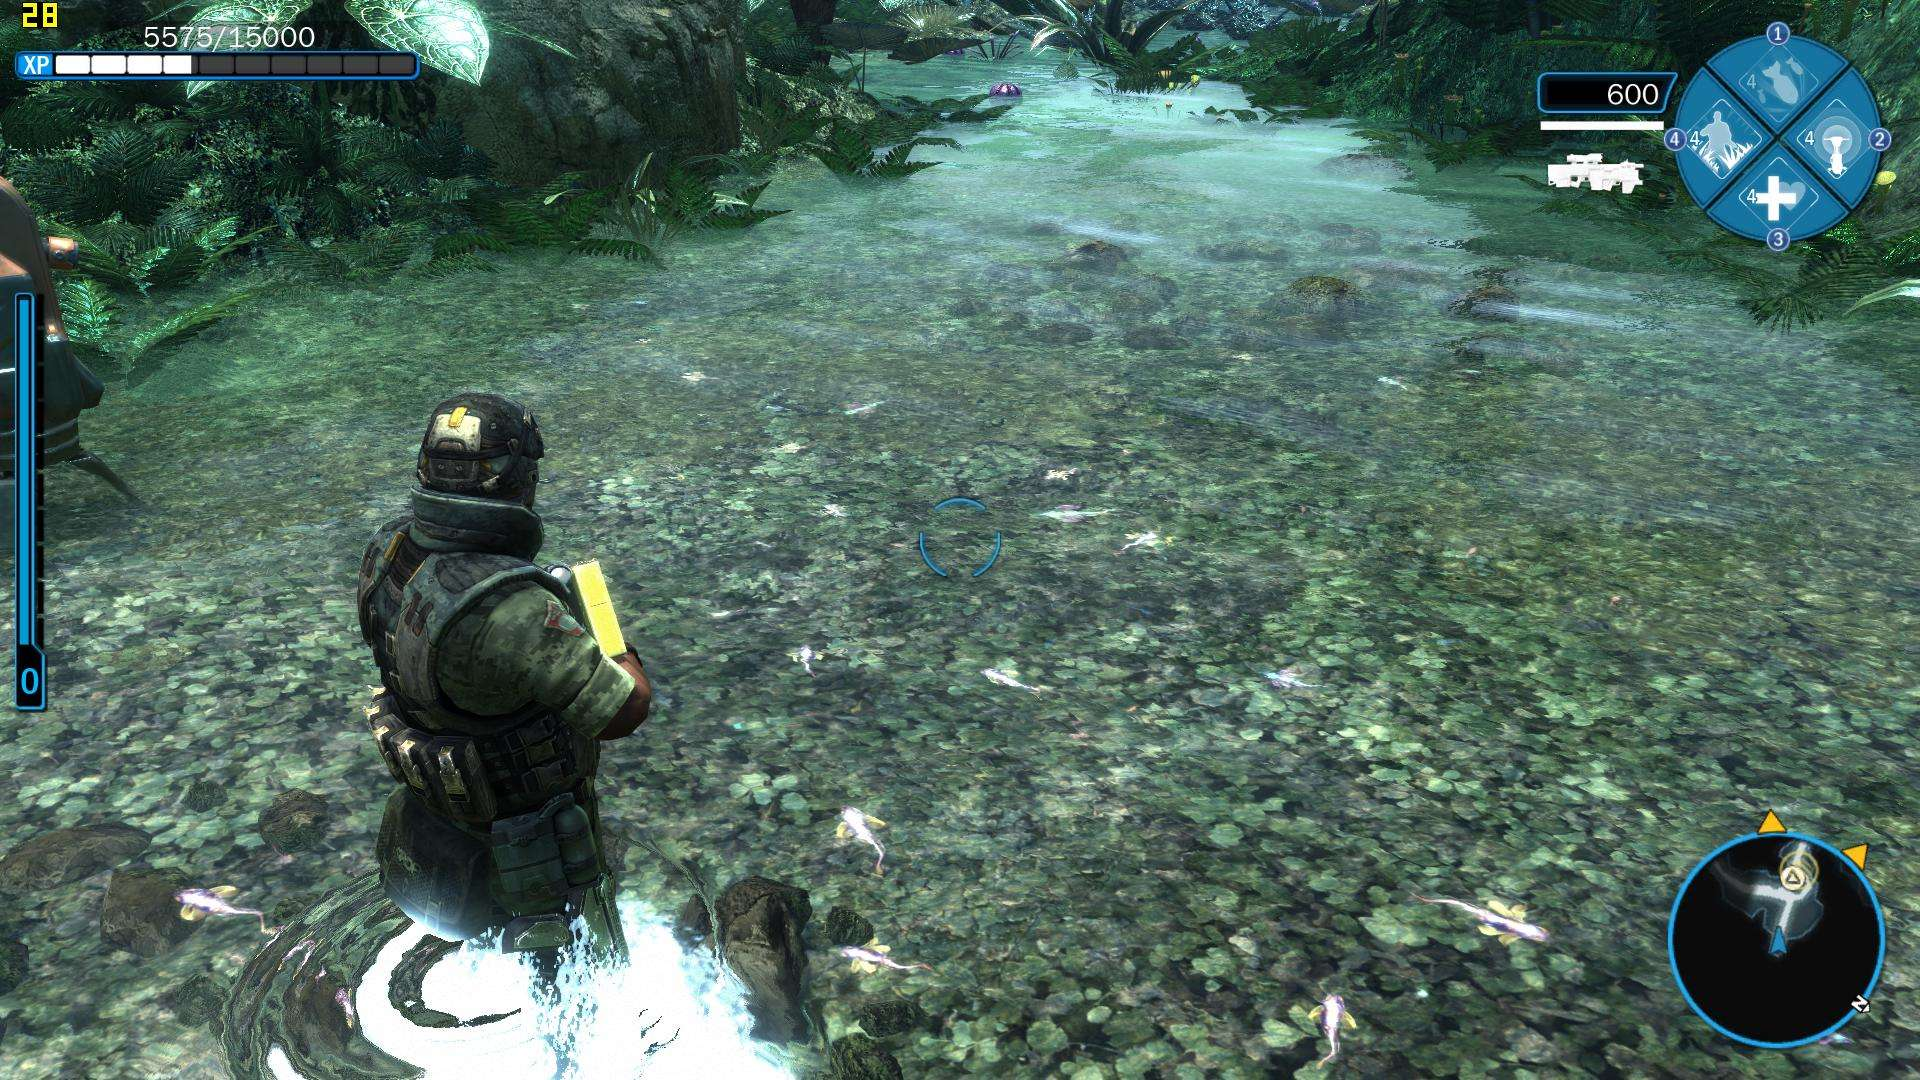
\includegraphics[width=1\textwidth]{figures/pic4.jpg}
        \subcaption*{3D games}
        \end{subfigure}
    }
    \caption*{\emph{Water simulation in games}}
  \label{fig:2}
  \end{figure}
\end{frame}

\begin{frame}{Applications}
  \begin{itemize}
    \item Research and industrial design
  \end{itemize}
  
  \begin{figure}[thpb]
    \centering
    \resizebox{0.5\linewidth}{!}{
        \centering
        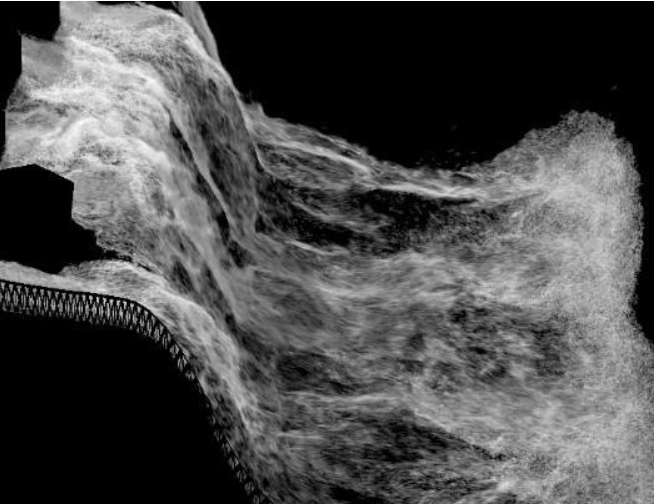
\includegraphics{figures/pic5.png}
    }
    \caption*{\emph{Flood model for dam design}}
  \label{fig:3}
  \end{figure}
\end{frame}
%%%%%%%%%%%%%%%%%%%%%%%%%%%%%%%%%%%%%%%%%%%%%%%%%%%%%%%%%%%%%%%%%%%%%%%%%%%%%%%%%
\begin{frame}{\emph{HOW} to simulate?}
  \textcolor[rgb]{0.5,0.5,0.5}{Quite difficult to deal with the \textbf{\color{blue}volatile} material...}
  \begin{columns}[T] % align columns
    \begin{column}<0->{.48\textwidth}
      \begin{figure}[thpb]
        \centering
        \resizebox{0.8\linewidth}{!}{
        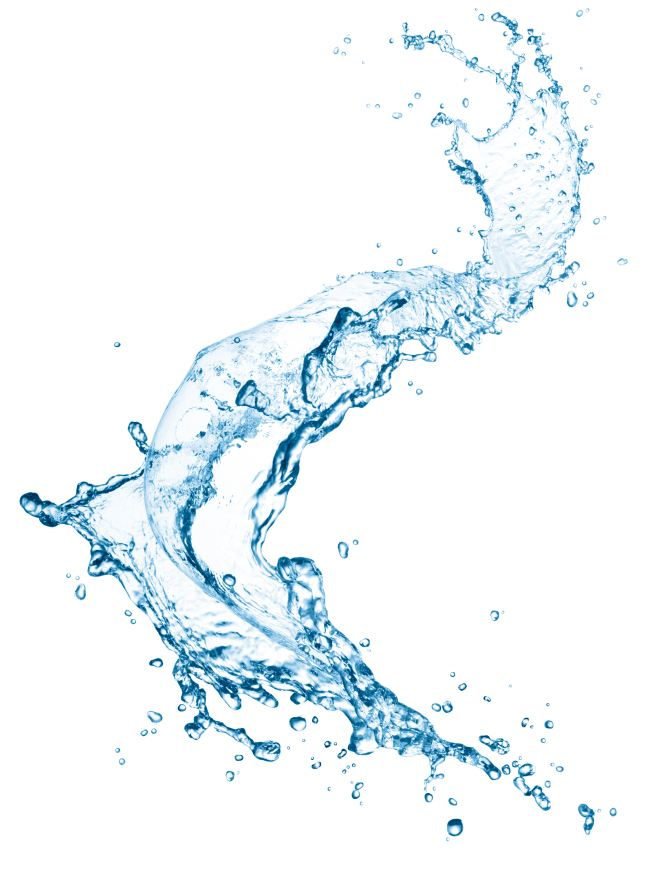
\includegraphics{figures/pic6.jpg}
        }
        %\includegraphics[scale=1.0]{figurefile}
        %\caption*{System components}
        \label{fig:system}
      \end{figure}
    \end{column}%
    \hfill%
    \begin{column}<0->{.58\textwidth}
      \\
      \small Three mainstream approaches:
      \begin{itemize}
      \setbeamertemplate{itemize items}{\color{red}$\bullet$}  
        \item Texture-based method : minimize the calculation, wildly used in real time rendering
          \begin{itemize}
            \setbeamertemplate{items}[ball]  
            \item Blinn, 1978, Bump Mapping
          \end{itemize}
        \item Construction-based method : more mathematicall
          \begin{itemize}
            \setbeamertemplate{items}[ball]  
            \item Cosine function superposition algorithm
            \item Gerstner Wave
            \item B-spline
          \end{itemize}
      \end{itemize}
    \end{column}%
  \end{columns}
\end{frame}
%%%%%%%%%%%%%%%%%%%%%%%%%%%%%%%%%%%%%%%%%%%%%%%%%%%%%%%%%%%%%%%%%%%%%%%%%%%%%%%%%
\begin{frame}{\emph{HOW} to simulate?}
  \textcolor[rgb]{0.5,0.5,0.5}{Quite difficult to deal with the \textbf{\color{blue}volatile} material...}
  \begin{columns}[T] % align columns
    \begin{column}<0->{.48\textwidth}
      \begin{figure}[thpb]
        \centering
        \resizebox{0.8\linewidth}{!}{
        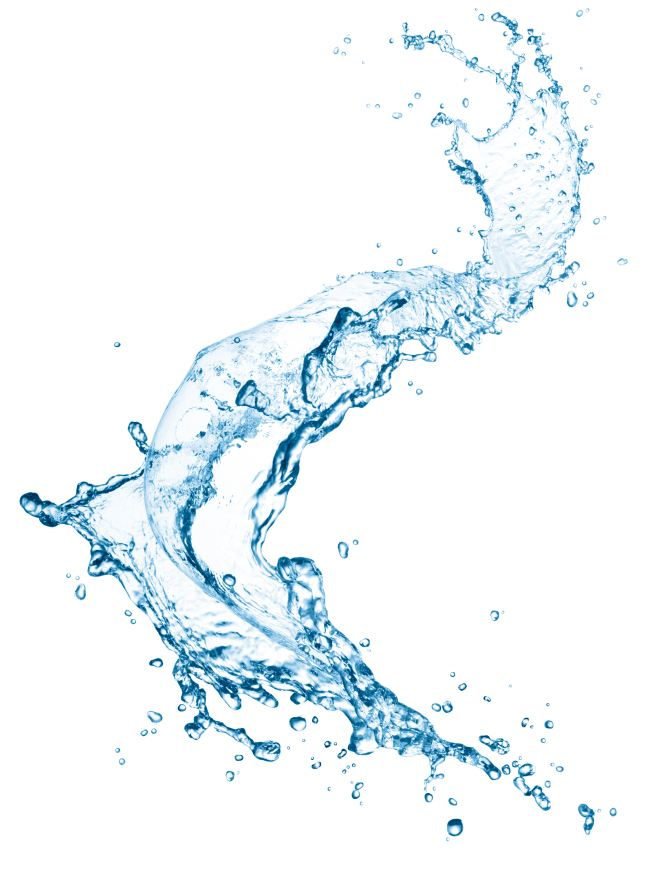
\includegraphics{figures/pic6.jpg}
        }
        %\includegraphics[scale=1.0]{figurefile}
        %\caption*{System components}
        \label{fig:system}
      \end{figure}
    \end{column}%
    \hfill%
    \begin{column}<0->{.58\textwidth}
      \\
      \begin{itemize}
      \setbeamertemplate{itemize items}{\color{red}$\bullet$}  
        \item Based on physics models : Realistic and Lifelike(pick it!\checkmark)
        \begin{figure}[thpb]
          \centering
          \resizebox{0.8\linewidth}{!}{
              \centering
              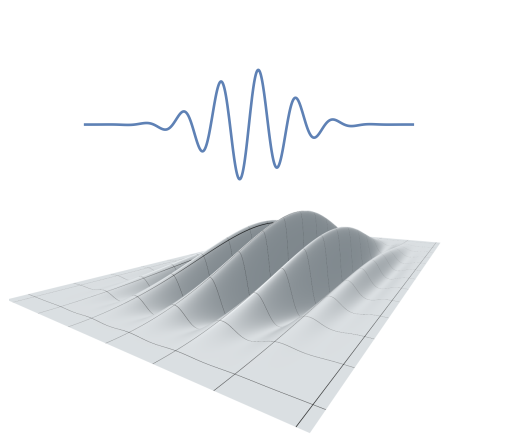
\includegraphics{figures/pic8.png}
          }
        \label{fig:system}
        \end{figure}
      \end{itemize}
    \end{column}%
  \end{columns}
\end{frame}
%%%%%%%%%%%%%%%%%%%%%%%%%%%%%%%%%%%%%%%%%%%%%%%%%%%%%%%%%%%%
\begin{frame}{Texture-based method : Bump Mapping}
  \textcolor[rgb]{0.5,0.5,0.5}{\large \textcolor[rgb]{1,0,0}{\textbf{\emph{"FAKE"}}} wave!!}
  \par Normal texture mapping \textcolor[rgb]{0,0.6,0.8}{\emph{does not change the shape of objects}}, but produces uneven effects.

  \begin{figure}[thpb]
    \centering
    \resizebox{0.5\linewidth}{!}{
        \centering
        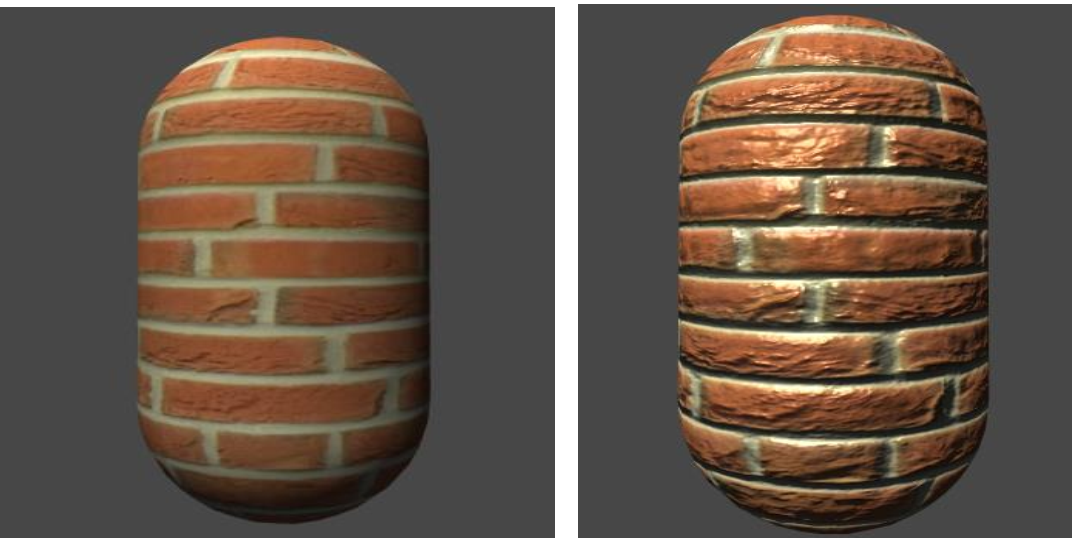
\includegraphics{figures/pic7.png}
    }
    \caption*{\emph{Normal texture mapping \textcolor[rgb]{0,0,1}{vs.} Bump mapping}}
  \label{fig:system}
  \end{figure}
\end{frame}
%%%%%%%%%%%%%%%%%%%%%%%%%%%%%%%%%%%%%%%%%%%%%%%%%%%%%%%%%%%
\begin{frame}{Texture-based method : Bump Mapping}
  How to store the normal map?
  \begin{itemize}
    \item In model space
    \item In tangent space(切线空间)
  \end{itemize}

  \begin{figure}[thpb]
    \centering
    \resizebox{0.3\linewidth}{!}{
        \centering
        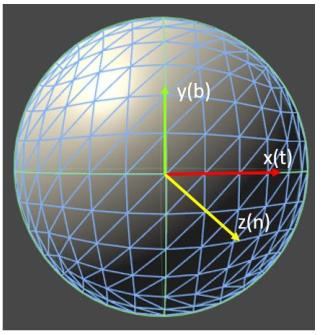
\includegraphics{figures/pic9.png}
    }
    \caption*{\emph{The tangent space of the vertices of a model}}
  \label{fig:system}
  \end{figure}
\end{frame}
%%%%%%%%%%%%%%%%%%%%%%%%%%%%%%%%%%%%%%%%%%%%%%%%%%%%%%%%%%
\begin{frame}{Texture-based method : Bump Mapping}
  To apply bump mapping in wave simulation, we should store
  \begin{itemize}
    \item Normal vector of the vertex
    \item \textcolor[rgb]{0,0,1}{Tangent vector of the vertex}
    \item \textcolor[rgb]{0,0,1}{Binormal vector of the vetex(副法线向量)}
  \end{itemize}
  Steps:
  \begin{enumerate}
    \item 在片元着色器中根据UV坐标对法线纹理进行采样,并还原真正的法线信息
    \item 利用矩阵M将光源方向以及视线方向从世界空间转换到切线空间,
          或者利用矩阵M的逆转置矩阵将法线从切线空间转换到世界空间
    \item 根据光照方程计算该片元的颜色
    \item 更新每个点的UV坐标,回到步骤1
  \end{enumerate}
\end{frame}
%%%%%%%%%%%%%%%%%%%%%%%%%%%%%%%%%%%%%%%%%%%%%%%%%%%%%%%%%%%%
\begin{frame}{Texture-based method : Bump Mapping}
  The core issue of the algorithm:  Constantly update the UV coordinates, then map the texture and calculate the light, so that the water appears to be fluctuating.
  \begin{itemize}
    \item \textcolor[rgb]{0,0,1}{\large Just \textcolor[rgb]{1,0,0}{\textbf{\emph{deceive}}} your eyes!}
    \item \textcolor[rgb]{0,0,1}{\textbf{Minumize} the calculation, effective in many cases.}
  \end{itemize}

  \begin{figure}[thpb]
    \centering
    \resizebox{0.3\linewidth}{!}{
        \centering
        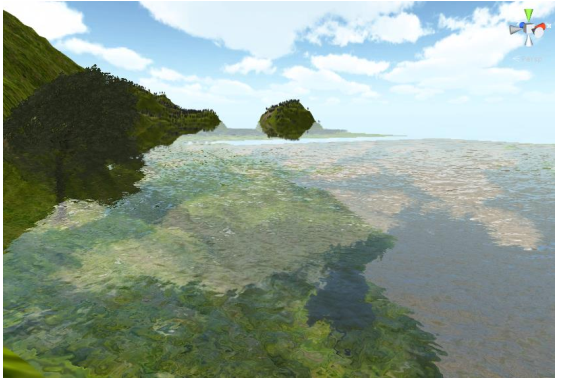
\includegraphics{figures/pic10.png}
    }
    \caption*{\emph{Applying bump mapping in water simulation}}
  \label{fig:system}
  \end{figure}
\end{frame}
%%%%%%%%%%%%%%%%%%%%%%%%%%%%%%%%%%%%%%%%%%%%%%%%%%%%%%%%%%%
\begin{frame}{Construction-based method}
  \begin{itemize}
    \item Cosine function superposition algorithm(余弦函数叠加法)
    \item Gerstner wave
    \item Fast Fourier transform(FFT)
    \item ...
  \end{itemize}
\end{frame}
%%%%%%%%%%%%%%%%%%%%%%%%%%%%%%%%%%%%%%%%%%%%%%%%%%%%%%%%%%%
\begin{frame}{Cosine function superposition algorithm(余弦函数叠加法)}
  Two main factors that influence the calculation of Fourier transform of the wave
    \begin{itemize}
      \item Gravity : $g$
      \item Surface tension(表面张力) : $\lambda$
    \end{itemize}
  And if the wavelength is long enough, the gravity plays the major role in the calculation.
\end{frame}
%%%%%%%%%%%%%%%%%%%%%%%%%%%%%%%%%%%%%%%%%%%%%%%%%%%%%%%%%%%
\begin{frame}{Cosine function superposition algorithm(余弦函数叠加法)}
  Using a nonlinear partial differential equation(NPDE) to describe the movement of the water surface, then we can got a approximate solution of the function
  \begin{figure}[thpb]
    \centering
    \resizebox{1\linewidth}{!}{
        \centering
        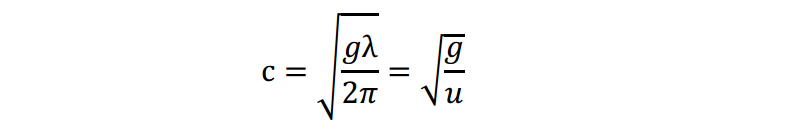
\includegraphics{figures/pic26.png}
    }
  \label{fig:system}
  \end{figure}
  where $u=\frac{2\pi}{\lambda}$ is the number of the waves, then we can describe the height of water surface as follow
  \begin{figure}[thpb]
    \centering
    \resizebox{1\linewidth}{!}{
        \centering
        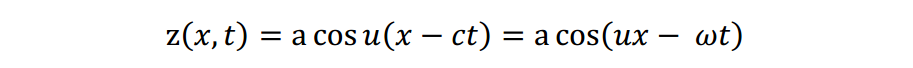
\includegraphics{figures/pic27.png}
    }
  \label{fig:system}
  \end{figure}
  print
\end{frame}
%%%%%%%%%%%%%%%%%%%%%%%%%%%%%%%%%%%%%%%%%%%%%%%%%%%%%%%%%%
\begin{frame}{Cosine function superposition algorithm(余弦函数叠加法)}
  $a$ is the amplitude(振幅), $/omega = uc$ is the angular velocity(角速度), in the 2-dimensional coordinate system
  \begin{figure}[thpb]
    \centering
    \resizebox{1\linewidth}{!}{
        \centering
        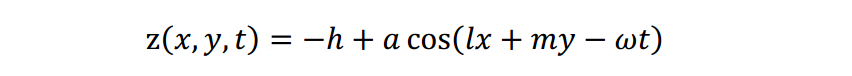
\includegraphics{figures/pic28.png}
    }
  \label{fig:system}
  \end{figure}
  h is the sea level height, since different waves that are independent
  \begin{figure}[thpb]
    \centering
    \resizebox{1\linewidth}{!}{
        \centering
        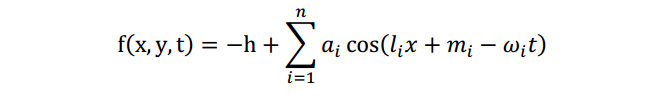
\includegraphics{figures/pic29.png}
    }
  \label{fig:system}
  \end{figure}
\end{frame}
#############################################################

\begin{frame}{Cosine function superposition algorithm(余弦函数叠加法)}
  \begin{figure}[thpb]
    \centering
    \resizebox{1\linewidth}{!}{
        \centering
        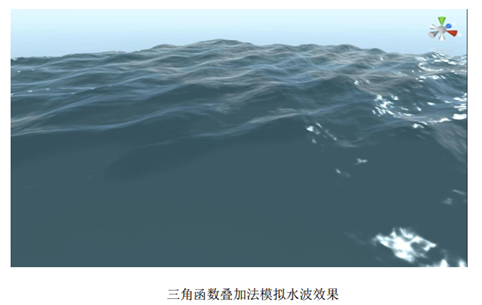
\includegraphics{figures/pic30.png}
    }
  \label{fig:system}
  \end{figure}
\end{frame}
%%%%%%%%%%%%%%%%%%%%%%%%%%%%%%%%%%%%%%%%%%%%%%%%%%%%%%%%%%
  
\begin{frame}{Based on physics models}
  Algorithms based on physics models can be divided into two categories
  \begin{itemize}
    \item Eulerian approache(grid-based)
    \item Lagrangian approache(based on particle system)
  \end{itemize}

  \begin{figure}[thpb]
    \centering
    \resizebox{0.7\linewidth}{!}{
        \centering
        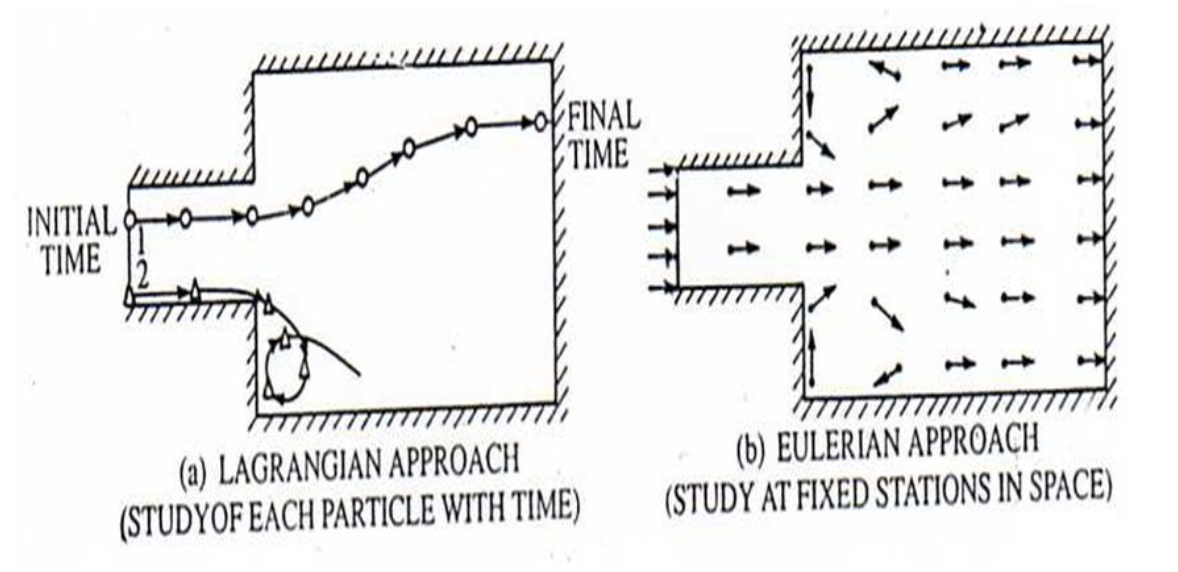
\includegraphics{figures/pic11.png}
    }
  \label{fig:system}
  \end{figure}
\end{frame}
%%%%%%%%%%%%%%%%%%%%%%%%%%%%%%%%%%%%%%%%%%%%%%%%%%%%%%%%%
\begin{frame}{Navier-Stokes(N-S) equation}
  \begin{figure}[thpb]
    \centering
    \resizebox{1\linewidth}{!}{
        \centering
        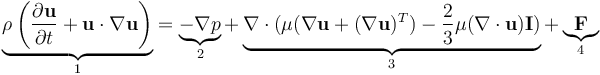
\includegraphics{figures/pic12.png}
    }
    %\caption*{\emph{N-S equation}}
  \label{fig:system}
  \end{figure}
  \textcolor[rgb]{0,0,1}{Drawbacks}
  \begin{itemize}
    \item Usually has no analytic solution
    \item Exponential time complexity !
  \end{itemize}
\end{frame}
%%%%%%%%%%%%%%%%%%%%%%%%%%%%%%%%%%%%%%%%%%%%%%%%%%%%%%%%%
\begin{frame}{Navier-Stokes(N-S) equation}
  To optimize...
  \begin{itemize}
    \item Make restriction to the conditions
      \begin{itemize}
        \item Hypothesis of small amplitude
        \item Hypothesis of shallow water[Kass and Miller 1990]
        \item Hypothesis of infinite depth of water[Mastin et al. 1987; Tessendorf 2004b]
        \item Ignore the solid boundary[Fournier and Reeves 1986]
      \end{itemize}
    \item Expore better numerical calculation Methods
      \begin{itemize}
        \item (Canabal et al. 2016)
        \item (Tessendorf 2004a)
      \end{itemize}
    \item More creative...
      \begin{itemize}
        \item Take the single wave as a whole research object in Lagrangian approache \textcolor[rgb]{0.7,0.7,0.5}{(instead of a single wave particle)} [Yuksel et al 2007]
      \end{itemize}
  \end{itemize}
\end{frame}
% -----------------------------------------------------------------------------
\section{Methods we have learnt}
\subsection{Methods we have learnt}

\begin{frame}{Overview of the article}
  \begin{itemize}
    \item Using the method 1 and 3 mentioned above
    \item Some novel work
      \begin{itemize}
        \item Introducing the concept of \textcolor[rgb]{0,0,1}{wave packet}
        \item Consider 5 visual verisimilitudes(视觉效果), including dispersion, refraction, reflection, diffraction and dissipation of water waves
        \item Parallelism and optimization
        \item Providing methods of adjusting parameters
      \end{itemize}
  \end{itemize}
\end{frame}
%%%%%%%%%%%%%%%%%%%%%%%%%%%%%%%%%%%%%%%%%%%%%%%%%%%%%%%%%%%%%%%%%%%%%
\begin{frame}{Some preparations!}
  \setbeamertemplate{blocks}[rounded][shadow=true]
  \setbeamercolor{block title}{fg=yellow,bg=blue!60!green}
  \setbeamercolor{block body}{bg=blue!20!white}
  \begin{block}{phase velocity(相速度) $c_p$}
    $3x10^9 m/s$, differentiated with 'group' velocity!
  \end{block}
  \begin{block}{wavenumber(波数) $k$}
    $k=\frac{2\pi}{\lambda}=\frac{2\pi f}{v}$, a descriptor of wave properties.
  \end{block}
\end{frame}
%%%%%%%%%%%%%%%%%%%%%%%%%%%%%%%%%%%%%%%%%%%%%%%%%%%%%%%%%%%%%%%%%%%%%
\begin{frame}{Some preparations!}
  \setbeamertemplate{blocks}[rounded][shadow=true]
  \setbeamercolor{block title}{fg=yellow,bg=blue!60!green}
  \setbeamercolor{block body}{bg=blue!20!white}
  \begin{block}{wave packets(波包)}
    一个石块扔进池塘引起的波纹不是一个波而是一组波,我们把这组波称为波包(Wave packets),其中每个波称为子波.
  \end{block}
  \begin{block}{group velocity(群速度)}
    用函数图像显示出来,下图中上面一行的就是两个子波,下面的则是他们形成的波包。整个波包移动的速度就是群速度.
  \end{block}

\end{frame}
%%%%%%%%%%%%%%%%%%%%%%%%%%%%%%%%%%%%%%%%%%%%%%%%%%%%%%%%%%%%%%%%%%%%%
\begin{frame}{Some preparations!}
  \begin{figure}[thpb]
    \centering
    \resizebox{1\linewidth}{!}{
        \centering
        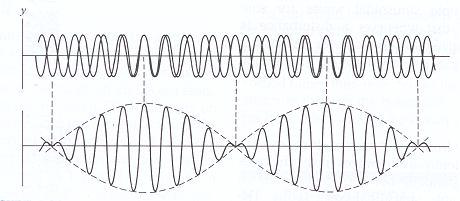
\includegraphics{figures/pic13.png}
    }
    %\caption*{\emph{N-S equation}}
  \label{fig:system}
  \end{figure}
\end{frame}
%%%%%%%%%%%%%%%%%%%%%%%%%%%%%%%%%%%%%%%%%%%%%%%%%%%%%%%%%%%%%%%%%
\begin{frame}{Some preparations!}
  \par 群速度的定义式如下,它等于某个子波的相速度加上$k$乘以相速度对$k$的偏导
  \begin{figure}[thpb]
    \centering
    \resizebox{0.7\linewidth}{!}{
        \centering
        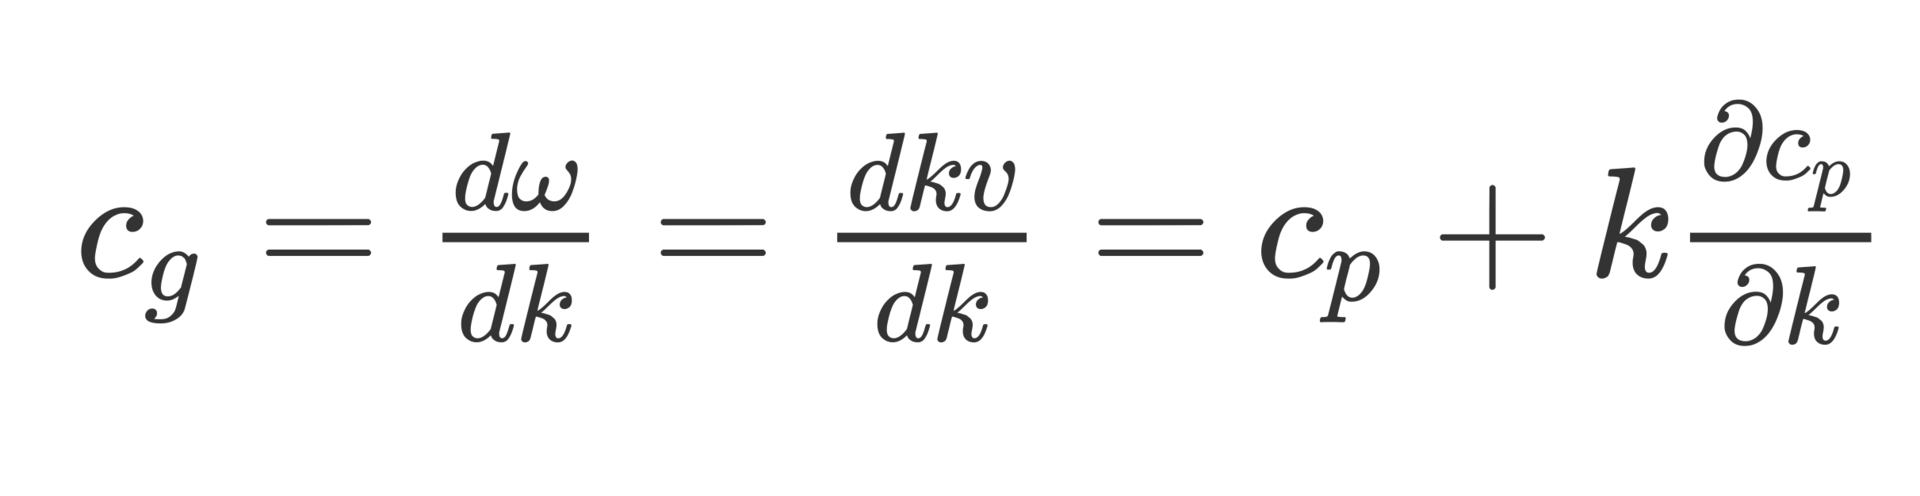
\includegraphics{figures/pic14.png}
    }
    %\caption*{\emph{N-S equation}}
  \label{fig:system}
  \end{figure}
\end{frame}
%%%%%%%%%%%%%%%%%%%%%%%%%%%%%%%%%%%%%%%%%%%%%%%%%%%%%%%%%%%%%%%%%
\begin{frame}{A personal analysis of this paper}
  How can we demonstrate \textbf{\textcolor[rgb]{0,0,1}{wave packts}}?
  \begin{itemize}
    \item Using Gauss Kernel Distribution(GKD, 高斯核分布) $e^_{-x^2}$ to represent a wave packet. $x$ is the space coordinates while on the surface of the water
  \end{itemize}
  \begin{figure}[thpb]
    \centering
    \resizebox{0.5\linewidth}{!}{
        \centering
        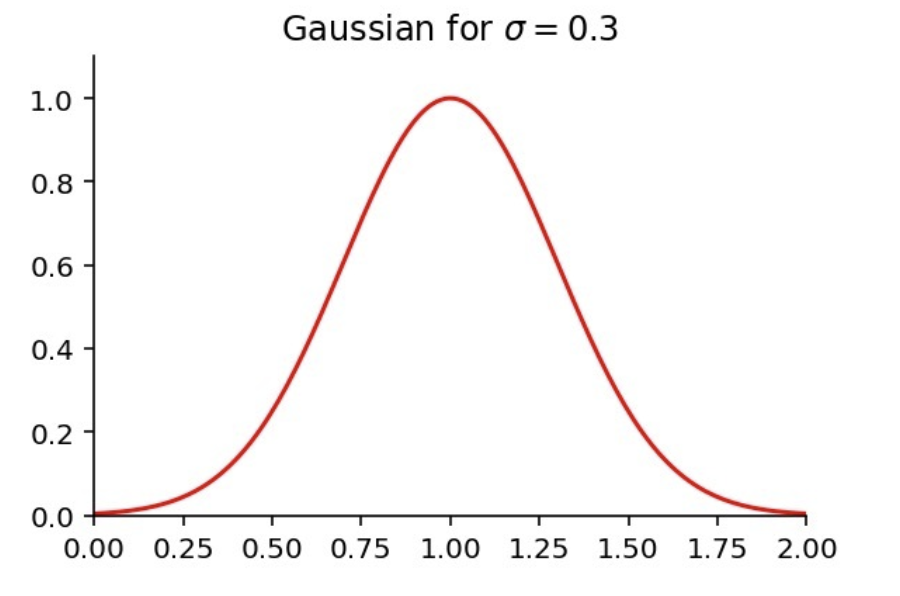
\includegraphics{figures/pic15.png}
    }
    \caption*{\emph{GKD function}}
  \label{fig:system}
  \end{figure}
\end{frame}
%%%%%%%%%%%%%%%%%%%%%%%%%%%%%%%%%%%%%%%%%%%%%%%%%%%%%%%%%%%%%%%%%
\begin{frame}{A personal analysis of this paper}
  Represent the wave packets...
  \begin{itemize}
    \item Amplitude(振幅) : $a_j$
    \item Wavenumber(波数) : $k_j$
    \item Wavelength(波长) : $\lambda_j$
  \end{itemize}
  \\
  \par 水面上,一个波包初始表示为一个前进方向长为3倍代表波长(Wavelength),正切方向长为6倍波长的矩形切片.
  \begin{figure}[thpb]
    \centering
    \resizebox{0.5\linewidth}{!}{
        \centering
        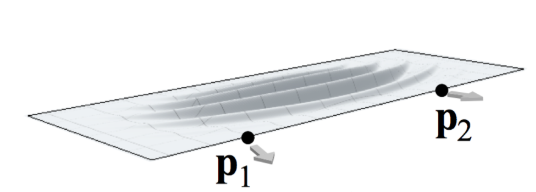
\includegraphics{figures/pic16.png}
    }
    \caption*{\emph{Represent a wave packet}}
  \label{fig:system}
  \end{figure}
\end{frame}
%%%%%%%%%%%%%%%%%%%%%%%%%%%%%%%%%%%%%%%%%%%%%%%%%%%%%%%%%%%%%%%%%
\begin{frame}{A personal analysis of this paper}
  波包运动过程中,两个点控制点的位置使用欧拉前项法迭代更新,下一时刻的位置等于前一时刻位置乘以波包的群速度
  \begin{figure}[thpb]
    \centering
    \resizebox{1\linewidth}{!}{
        \centering
        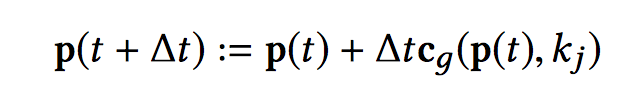
\includegraphics{figures/pic17.png}
    }
    %\caption*{\emph{Represent a wave packet}}
  \label{fig:system}
  \end{figure}
\end{frame}
%%%%%%%%%%%%%%%%%%%%%%%%%%%%%%%%%%%%%%%%%%%%%%%%%%%%%%%%%%%%%%%%%
\begin{frame}{A personal analysis of this paper}
  积分形式:积分变量是波数$k$,被积函数第一项$a(k)$代表一个波数为$k$的子波的振幅。直观上可以理解:\textcolor[rgb]{0,0,1}{点$x$处的水面高度是所有子波的振幅加权求和}.
  \begin{figure}[thpb]
    \centering
    \resizebox{1\linewidth}{!}{
        \centering
        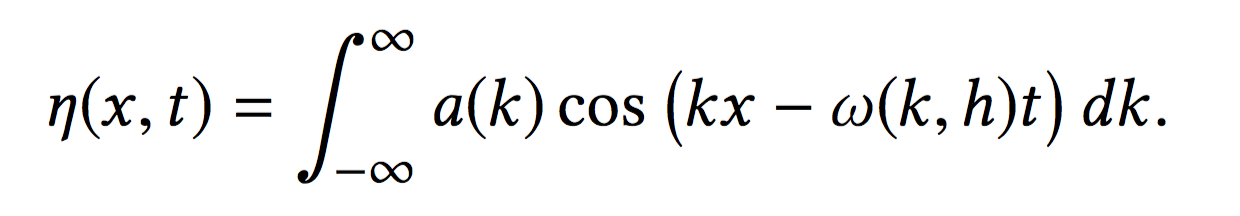
\includegraphics{figures/pic18.png}
    }
    %\caption*{\emph{Represent a wave packet}}
  \label{fig:system}
  \end{figure}
\end{frame}
%%%%%%%%%%%%%%%%%%%%%%%%%%%%%%%%%%%%%%%%%%%%%%%%%%%%%%%%%%%%%%%%%
\begin{frame}{A personal analysis of this paper}
  最后,假设在时刻$t$,水面点$x$重叠了$N$个波包,那么该点的高度就是这$N$个波包分别使用Airy波理论算出的水面高度之和. 公式如下: 通过该公式可以方便地计算出水面上任意点的高度,从而绘制出水面.
  \begin{figure}[thpb]
    \centering
    \resizebox{1\linewidth}{!}{
        \centering
        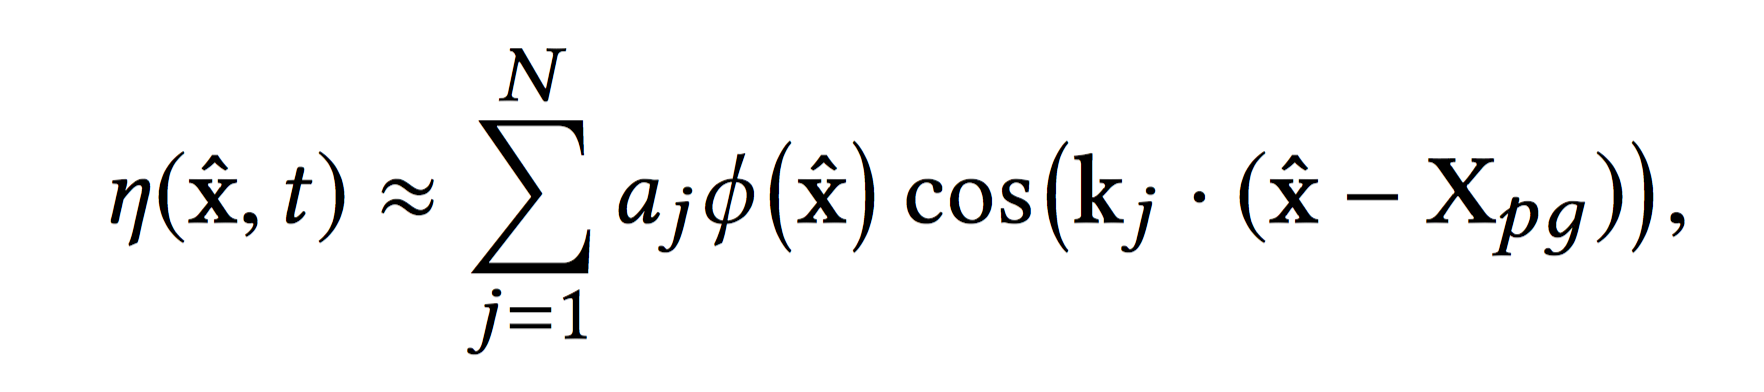
\includegraphics{figures/pic19.png}
    }
    %\caption*{\emph{Represent a wave packet}}
  \label{fig:system}
  \end{figure}
  \\ \emph{\large \centering \textbf{\textcolor[rgb]{0,0,1}{More clearly?}}}
\end{frame}
%%%%%%%%%%%%%%%%%%%%%%%%%%%%%%%%%%%%%%%%%%%%%%%%%%%%%%%%%%%%%%%%%
\begin{frame}{A personal analysis of this paper}
  How about dispersion(色散), refraction(折射), reflection(反射), diffraction(衍射) and energy loss(能量损失) of water waves?
  \setbeamertemplate{blocks}[rounded][shadow=true]
  \setbeamercolor{block title}{fg=yellow,bg=blue!60!green}
  \setbeamercolor{block body}{bg=blue!20!white}
  \begin{block}{dispersion(色散)}
    色散是指不同波长的波作为一个波包在传播中分散的现象.
  \end{block}
  \par 论文中使用两个控制点表示波包方向的做法自然地给出了实现这一现象的方法: 由于控制点P1P2与群速度不共线,因此当P1和P2不断更新迭代后其距离会不断拉大,达到3倍代表波长时就从几何中点$P_{sub}$处会分离,它们的几何中点$P_{sub}$,分别与$P_1$,$P_2$连成两个新的波包的前进方向的边.
  \\ \emph{\large \centering \textbf{\textcolor[rgb]{0,0,1}{Interesting!}}}
\end{frame}
%%%%%%%%%%%%%%%%%%%%%%%%%%%%%%%%%%%%%%%%%%%%%%%%%%%%%%%%%%%%%%%%%
\begin{frame}{A personal analysis of this paper}
  \begin{figure}[thpb]
    \centering
    \resizebox{0.9\linewidth}{!}{
        \centering
        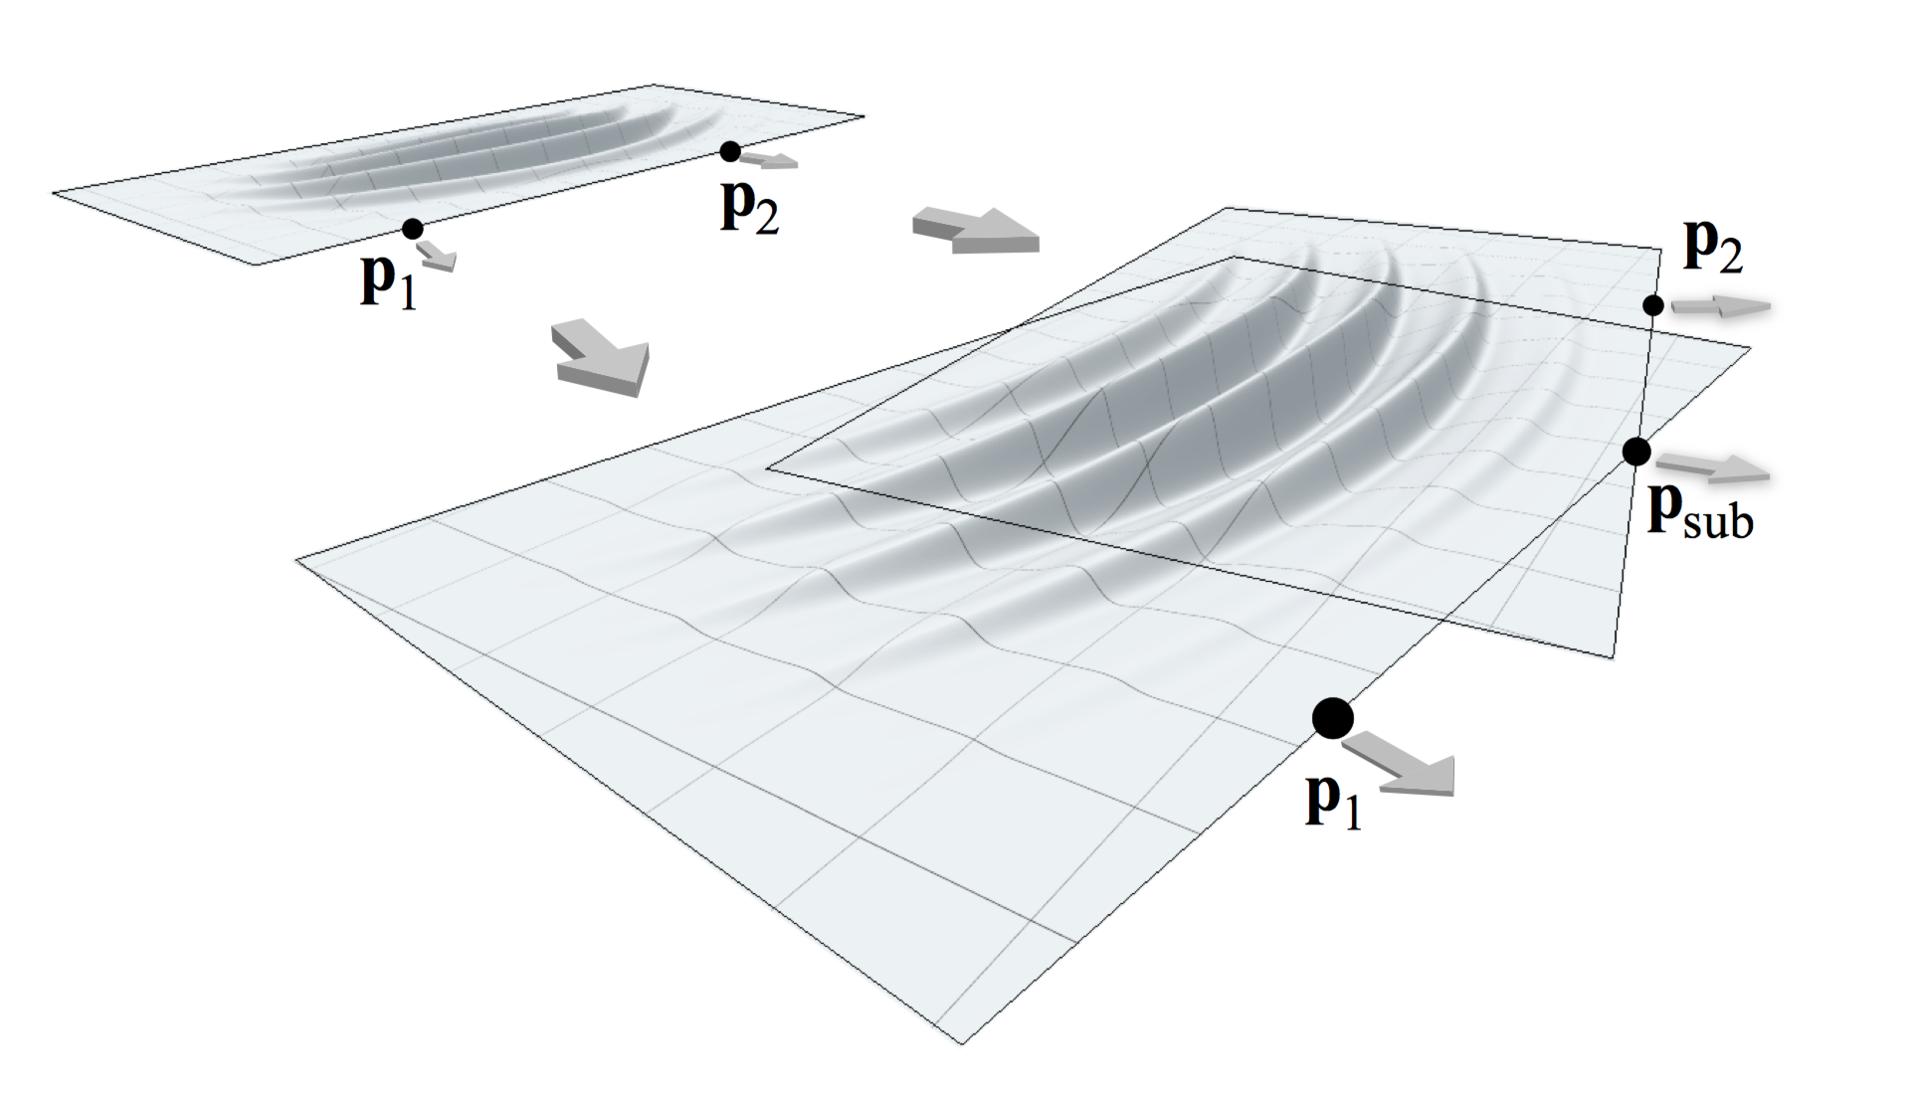
\includegraphics{figures/pic20.png}
    }
    \caption*{\emph{波包“分蘖”}}
  \label{fig:system}
  \end{figure}
\end{frame}
%%%%%%%%%%%%%%%%%%%%%%%%%%%%%%%%%%%%%%%%%%%%%%%%%%%%%%%%%%%%%%%%%
\begin{frame}{A personal analysis of this paper}
  \setbeamertemplate{blocks}[rounded][shadow=true]
  \setbeamercolor{block title}{fg=yellow,bg=blue!60!green}
  \setbeamercolor{block body}{bg=blue!20!white}
  \begin{block}{refraction(折射)}
    折射是由于在水面波通过不同深度的水域时,其群速度会发生改变,由惠更斯定理(Huygens theorem)可算出折射后的速度方向.
  \end{block}
  
  \begin{figure}[thpb]
    \centering
    \resizebox{0.6\linewidth}{!}{
        \centering
        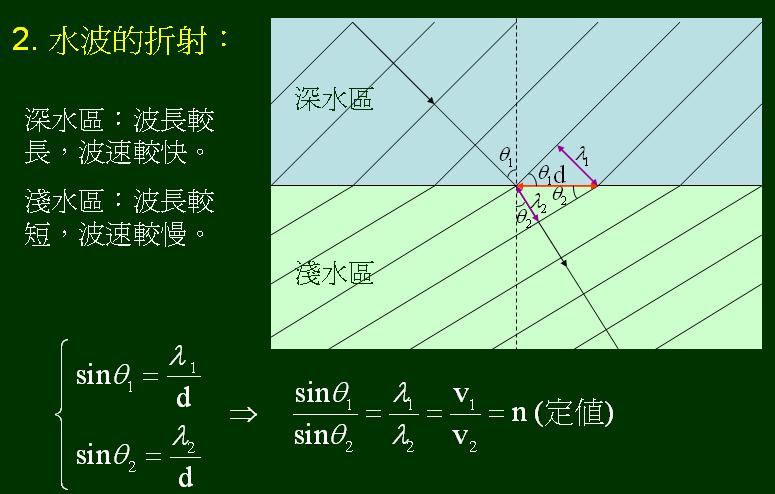
\includegraphics{figures/pic21.jpg}
    }
  \label{fig:system}
  \end{figure}
\end{frame}
%%%%%%%%%%%%%%%%%%%%%%%%%%%%%%%%%%%%%%%%%%%%%%%%%%%%%%%%%%%%%%%%%
\begin{frame}{A personal analysis of this paper}
  The paper just used the normal reflection theorem to simulate reflection, quite reasonable.
  
  \setbeamertemplate{blocks}[rounded][shadow=true]
  \setbeamercolor{block title}{fg=yellow,bg=blue!60!green}
  \setbeamercolor{block body}{bg=blue!20!white}
  \begin{block}{diffraction(衍射)}
    波的衍射是指波遇到障碍物后偏离原来的运动方向的现象.
  \end{block}
  In this paper, the method of diffraction is to show the effect of "sticking" on obstacles(粘附障碍物) after wave meets obstacles.
\end{frame}
%%%%%%%%%%%%%%%%%%%%%%%%%%%%%%%%%%%%%%%%%%%%%%%%%%%%%%%%%%%%%%%%%
\begin{frame}{A personal analysis of this paper}

\begin{figure}[thpb]
    \centering
    \resizebox{0.8\linewidth}{!}{
        \centering
        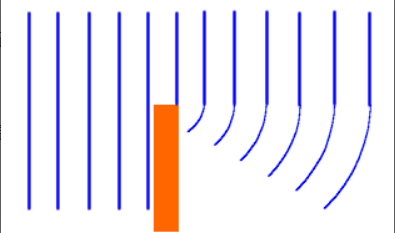
\includegraphics{figures/pic22.png}
    }
  \label{fig:system}
  \end{figure}
\end{frame}
%%%%%%%%%%%%%%%%%%%%%%%%%%%%%%%%%%%%%%%%%%%%%%%%%%%%%%%%
\begin{frame}{A personal analysis of this paper}
  Let's focus on the energy loss now!
  \\由于水的黏着性等因素,水面波会发生能量耗散,并使得振幅随时间降低,最终降为0。这一过程可以用下面这个对振幅的迭代方程表示:
  \begin{figure}[thpb]
    \centering
    \resizebox{0.8\linewidth}{!}{
        \centering
        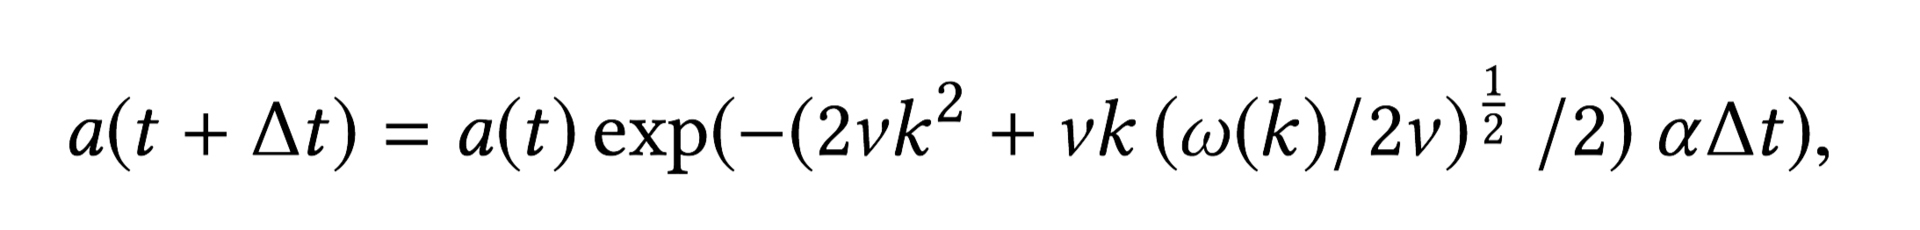
\includegraphics{figures/pic23.png}
    }
  \label{fig:system}
  \end{figure}
  其中$\alpha$被称为阻尼系数,$\alpha$越大,水波耗散地越快
\end{frame}
%%%%%%%%%%%%%%%%%%%%%%%%%%%%%%%%%%%%%%%%%%%%%%%%%%%%%%%%
\begin{frame}{A personal analysis of this paper}
  Something other things : How do authors accelerate the calculation and make optimization?
  \begin{itemize}
    \item 程序GPU加速,并行地计算出水面网格上各点的高度
    \item 波包设置上限,通过动态调整\textcolor[rgb]{0,0,1}{阻尼系数}使播报数量稳定在上限附近
  \end{itemize}
\end{frame}
%%%%%%%%%%%%%%%%%%%%%%%%%%%%%%%%%%%%%%%%%%%%%%%%%%%%%%%%
\begin{frame}{A personal analysis of this paper}
  Last but not least...
  \\How to generate different form of water waves by adjusting the speed of wave sources?
  \\波源指引发波的物体,例如一个移动中的小船,它某一时刻的运动引发的波的波数可以由开尔文定理给出:公式中v是这一时刻小船的速度,$\theta$是波包群速度方向和小船运动方向的夹角.

  \begin{figure}[thpb]
    \centering
    \resizebox{0.8\linewidth}{!}{
        \centering
        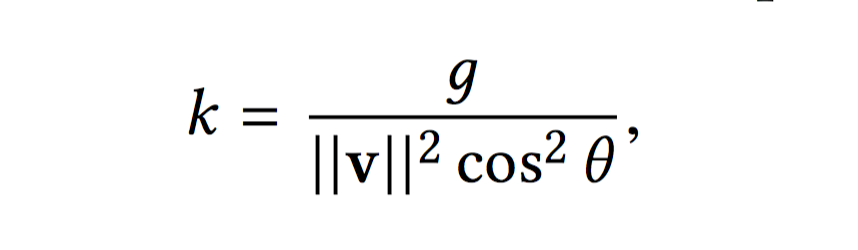
\includegraphics{figures/pic24.png}
    }
  \label{fig:system}
  \end{figure}
\end{frame}
%%%%%%%%%%%%%%%%%%%%%%%%%%%%%%%%%%%%%%%%%%%%%%%%%%%%%%%%%%%%%%%%%
\begin{frame}{A personal analysis of this paper}
  For example, adjust $v$, we can simulate the different effect of a swimming duck and a working ship.

  \begin{figure}[thpb]
    \centering
    \resizebox{0.5\linewidth}{!}{
        \centering
        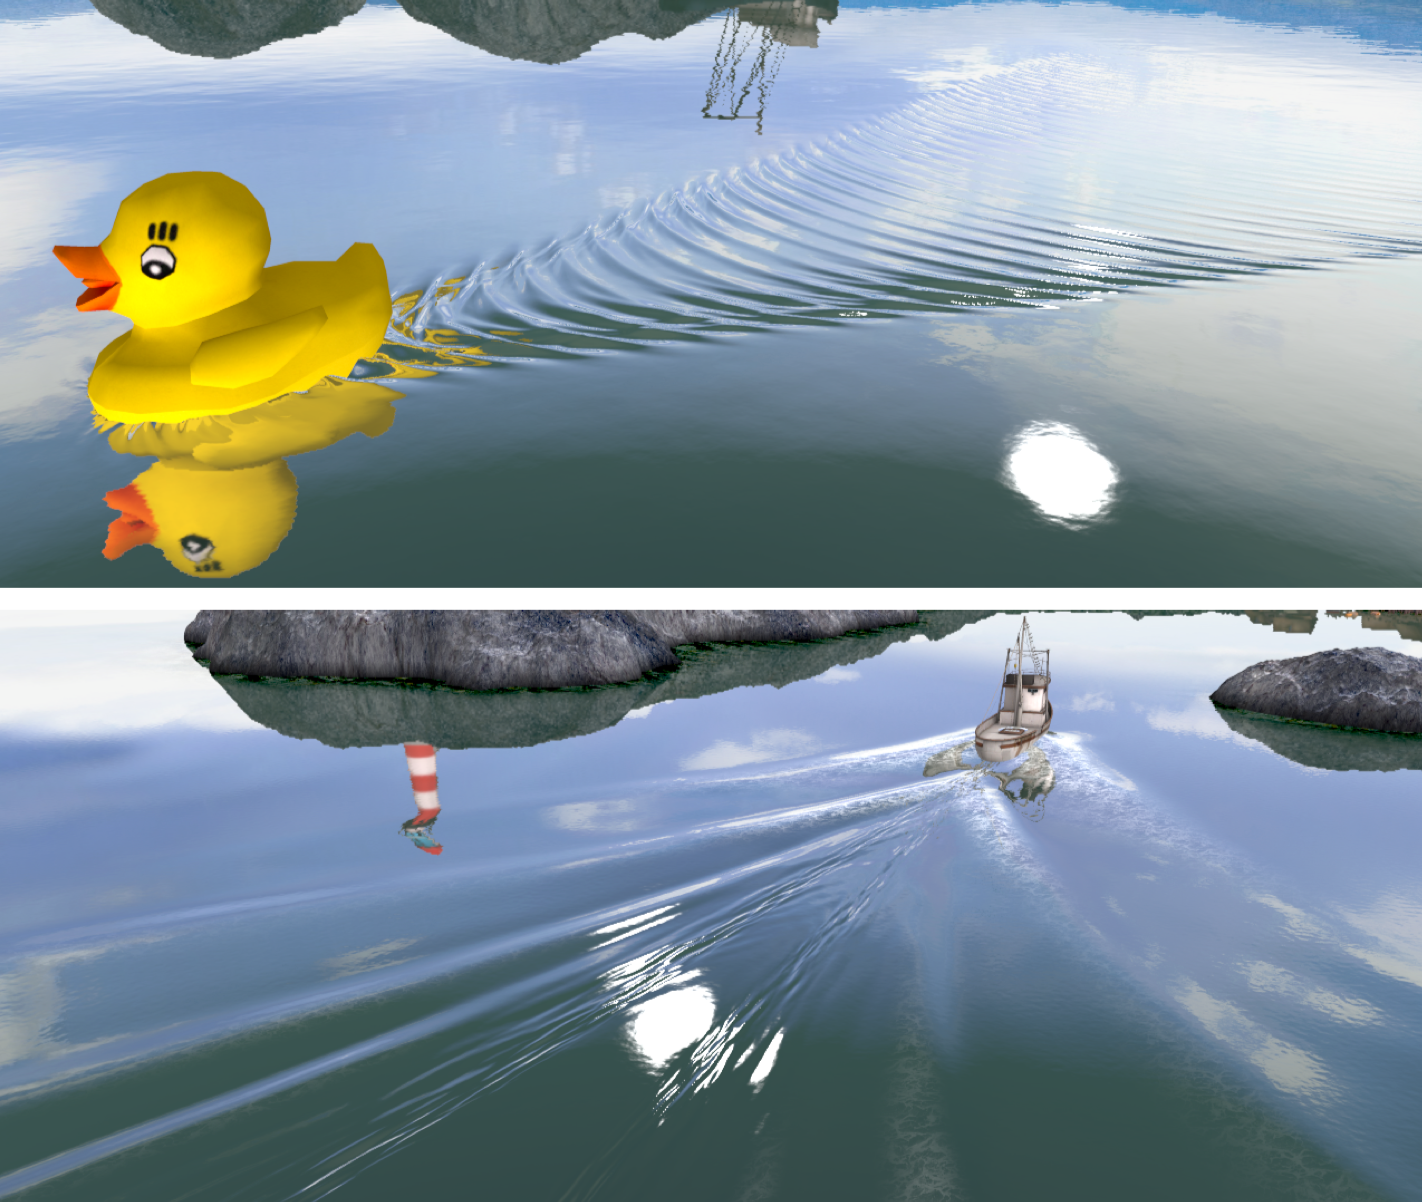
\includegraphics{figures/pic25.png}
    }
  \label{fig:system}
  \end{figure}
 \end{frame}
% -----------------------------------------------------------------------------
\section{A fun demo}
\subsection{A fun demo}
\begin{frame}{Demo}
  \centering
  \Huge \textbf{\textcolor[rgb]{0,0,1}{Now is the demo time!}}
\end{frame}

\begin{frame}{Group member}
 \large
  \begin{center}
    \begin{tabular}{cc}%
    李新锐\ 15323032&孙一言\ 16337216\\
    王锦鹏\ 16337232&王永锋\ 16337237\\
    颜彬\ 16337269&韦博耀\ 16337242
    \end{tabular}
  \end{center}
\end{frame}

\begin{frame}{Thank you}
  \begin{center}
    \Huge Thank you for listening!
  \end{center}
\end{frame}
% -----------------------------------------------------------------------------
\end{document}
